\section{back-up script}

%\begin{figure*}[!h]
%	\centering
%	\subfloat[PV Generation  ]{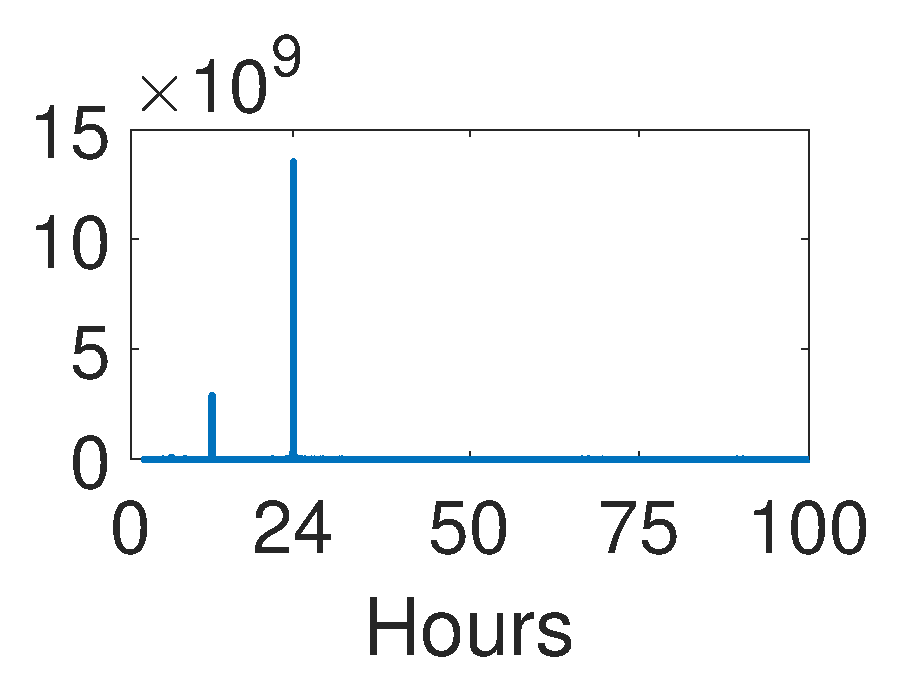
\includegraphics[width=.3\linewidth]{figs/solar_periodogram_al}}
%	\subfloat[Wind Generation]{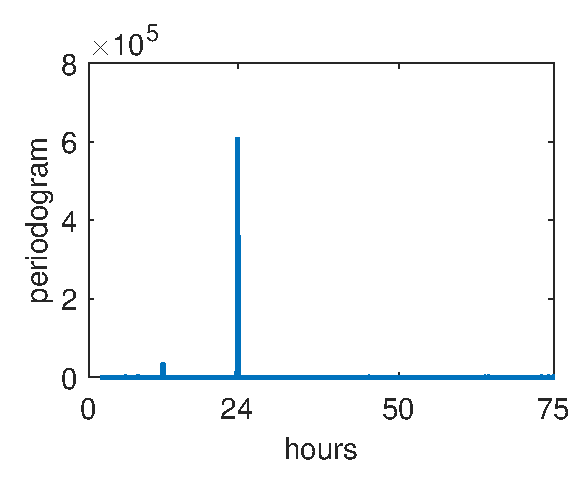
\includegraphics[width=.3\linewidth]{figs/wind_periodogram}}
%%	\subfloat[Price          ]{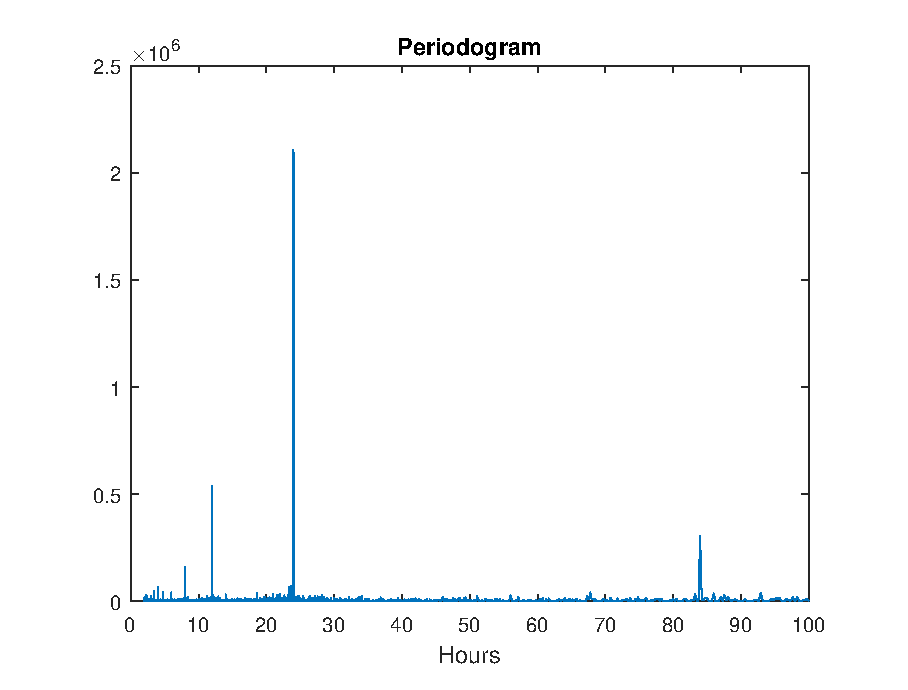
\includegraphics[width=.3\linewidth]{figs/price_periodogram_sanjose}}
%	%\subfloat[Workload       ]{\includegraphics[width=.2\linewidth]{figs/rosette}}
%	\caption{The periodograms of of PV generation (a), Wind generation (b), Electricity prices (c), and workload (d).}
%	\label{fig:periodgram}
%\end{figure*}


%The regression models, such as autoregressive model (AR), moving average model (MA), autoregressive moving average model (ARMA), and autoregressive integrated moving average model (ARIMA) have been used in predicting wind power or solar power \cite{guoyang2005discussion, kamal1997time, bacher2009online}. Kalman filtering, which is suitable for online forecasting, was used in predicting of wind speed \cite{louka2008improvements, costa2008review}. The solar irradiance in partly cloudy day is predicted by using Kalman filtering \cite{hassanzadeh2010practical}. Machine learning techniques are widely applied in forecasting solar and wind power. artificial neural network (ANN) is known as the best method among machine learning techniques due to its ability of deriving the meaning from complicated data \cite{paoli2010forecasting, sfetsos2000univariate}.
%Bacher et al. evaluated AR models in forecasting solar power up to 2 hour ahead \cite{bacher2009online}. ARMA models are used to predict 3 hour ahead solar generation in a lab based microgrid and achieve small errors in short term \cite{huang2012solar}. Kalman filtering, which is suitable for online forecasting, was used in predicting of wind speed \cite{louka2008improvements, costa2008review}. The solar irradiance in partly cloudy day is predicted by using Kalman filtering \cite{hassanzadeh2010practical}. Machine learning techniques are widely applied in forecasting solar and wind power. artificial neural network (ANN) is known as the best method among machine learning techniques due to its ability of deriving the meaning from complicated data. multi-layer perceptron (MLP) network \cite{paoli2010forecasting}. Sfetsos et al. developed an artificial intelligence model to predict the solar radiation received by the global surface  \cite{sfetsos2000univariate}. The results showed that the artificial intelligence models predict the solar radiation time series more effectively than the conventional time series methods. Martin et al. presented the performance comparison of AR, ANN, and fuzzy network based methods \cite{martin2010prediction}. The comparisons show that the ANN and fuzzy network based methods can obtain better results from lost component in the time series than AR models.

%Most of the physical methods take physical conditions as the input of their models and mainly based on machine learning techniques. The latitude, longitude, and duration of sunshine are input into the ANN models to predict solar radiation of 5 sites in Malaysia \cite{khatib2011modeling}. From weather forecast data, Navin Sharma et al. predict the total amount of solar generation a day ahead \cite{sharma2011predicting}. Generally, the physical methods may have more accurate output than the statistical methods; however, they physical methods significantly depend on the accuracy of physical condition, such as weather forecast data.

%\begin{figure*}[!h]
%	\centering
%	\subfloat[PV Generation  ]{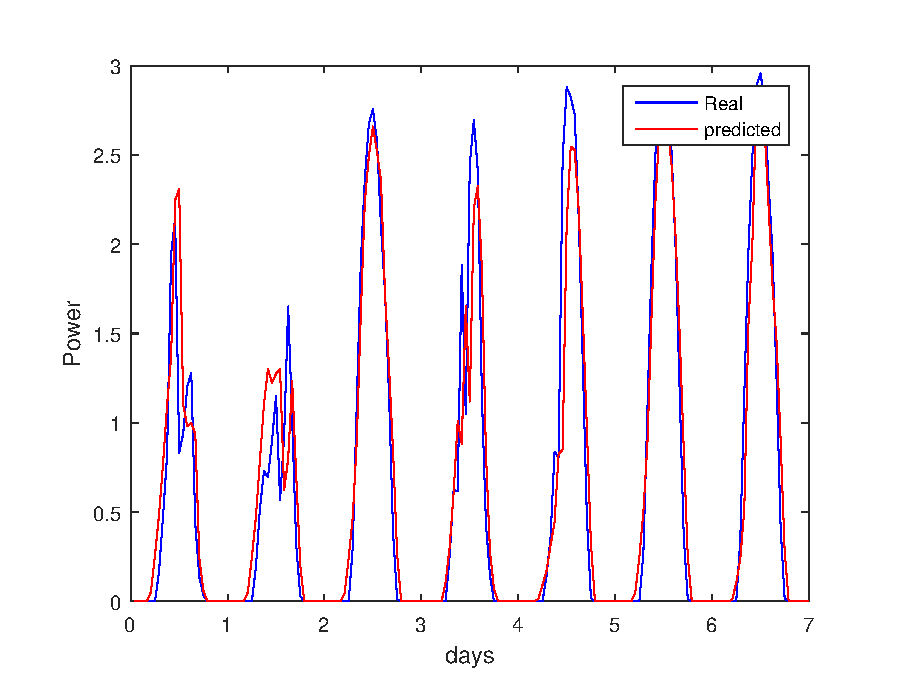
\includegraphics[width=.3\linewidth]{figs/solar_ar_adv}}
%	\subfloat[Wind Generation]{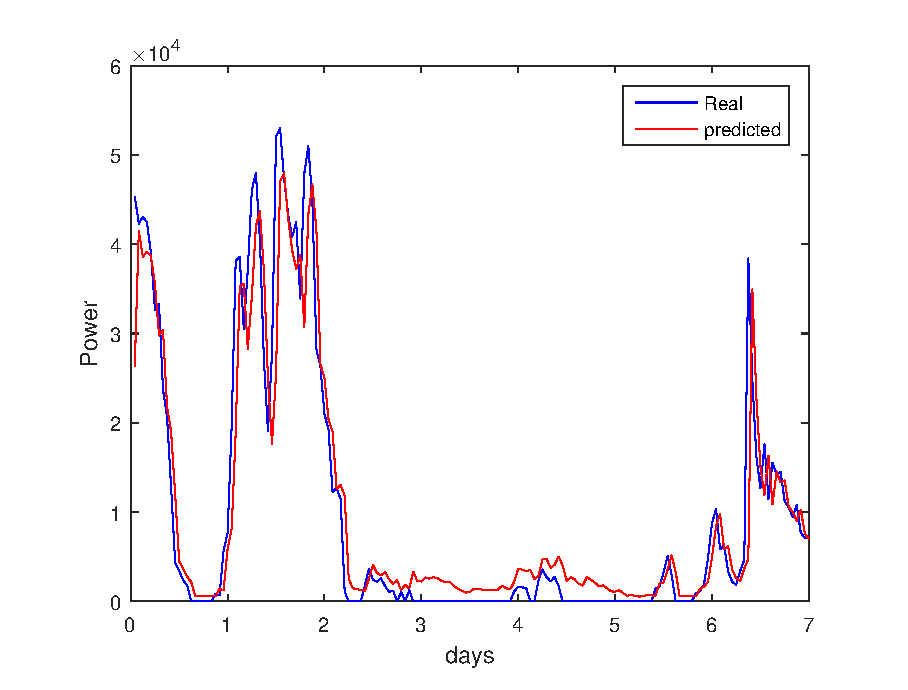
\includegraphics[width=.3\linewidth]{figs/wind_ar_adv}}
%	\subfloat[Price          ]{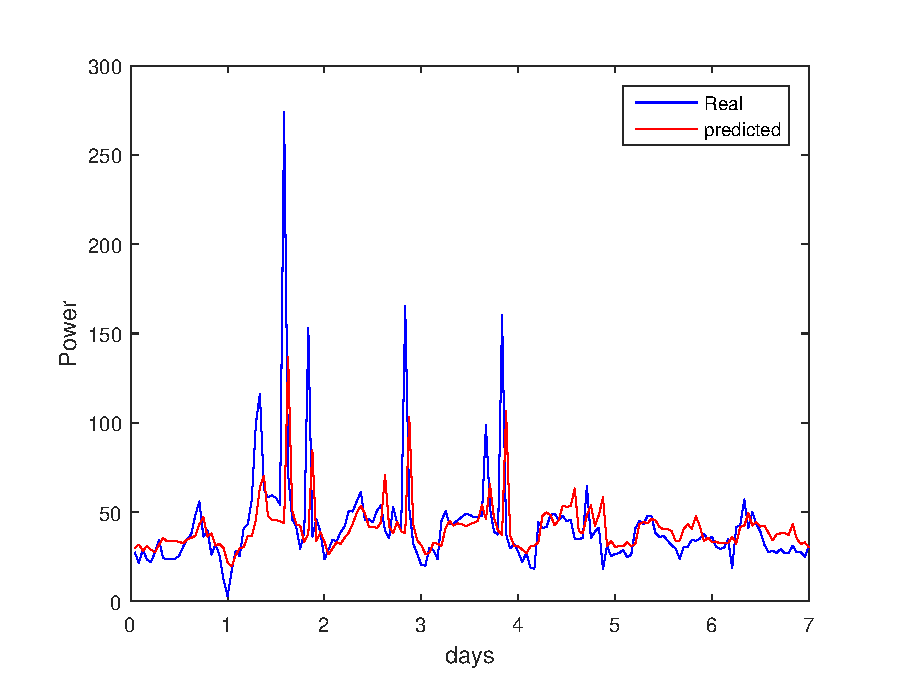
\includegraphics[width=.3\linewidth]{figs/price_ar_adv}}
%	%\subfloat[Workload       ]{\includegraphics[width=.2\linewidth]{figs/rosette}}
%	\caption{1 hour ahead AR prediction of PV generation (a), Wind generation (b), Electricity prices (c), and workload (d).}
%	\label{fig:periodgram}
%\end{figure*}
%
%\begin{figure*}[!h]
%	\centering
%	\subfloat[PV Generation  ]{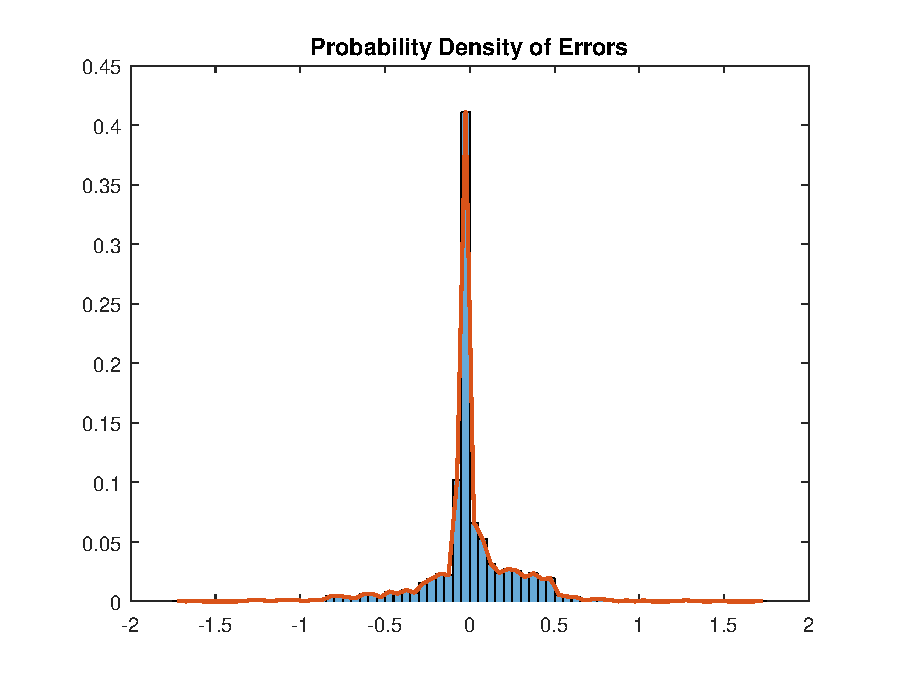
\includegraphics[width=.3\linewidth]{figs/solar_ar_adv_pdf}}
%	\subfloat[Wind Generation]{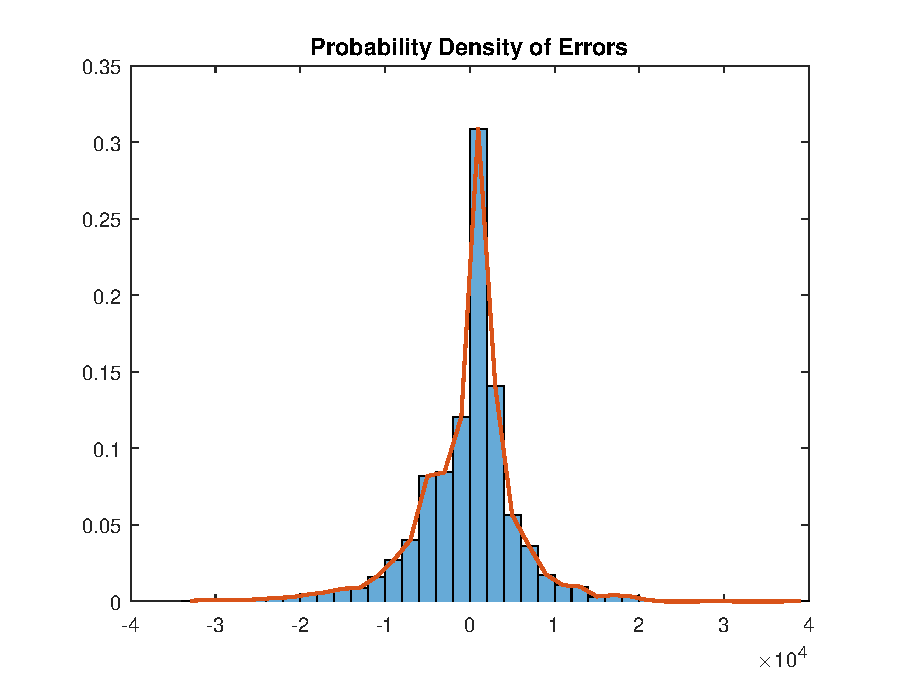
\includegraphics[width=.3\linewidth]{figs/wind_ar_adv_pdf}}
%	\subfloat[Price          ]{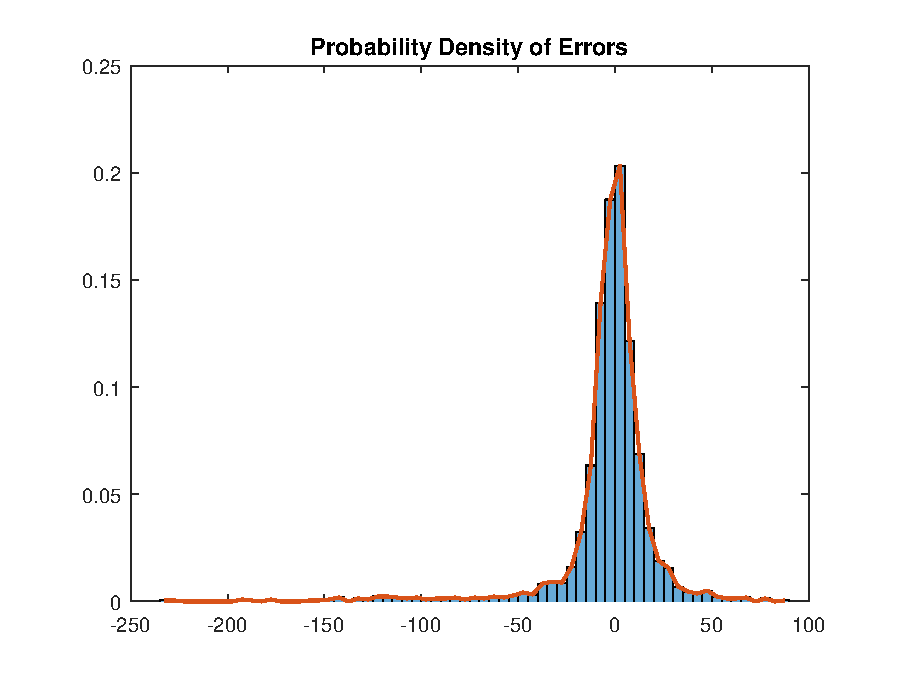
\includegraphics[width=.3\linewidth]{figs/price_ar_adv_pdf}}
%	%\subfloat[Workload       ]{\includegraphics[width=.2\linewidth]{figs/rosette}}
%	\caption{pdf(probability desity function) of 1 hour ahead AR prediction errors for PV generation (a), Wind generation (b), Electricity prices (c), and workload (d).}
%	\label{fig:periodgram}
%\end{figure*}

%\begin{figure*}[!h]
%	\centering
%	\subfloat[PV Generation  ]{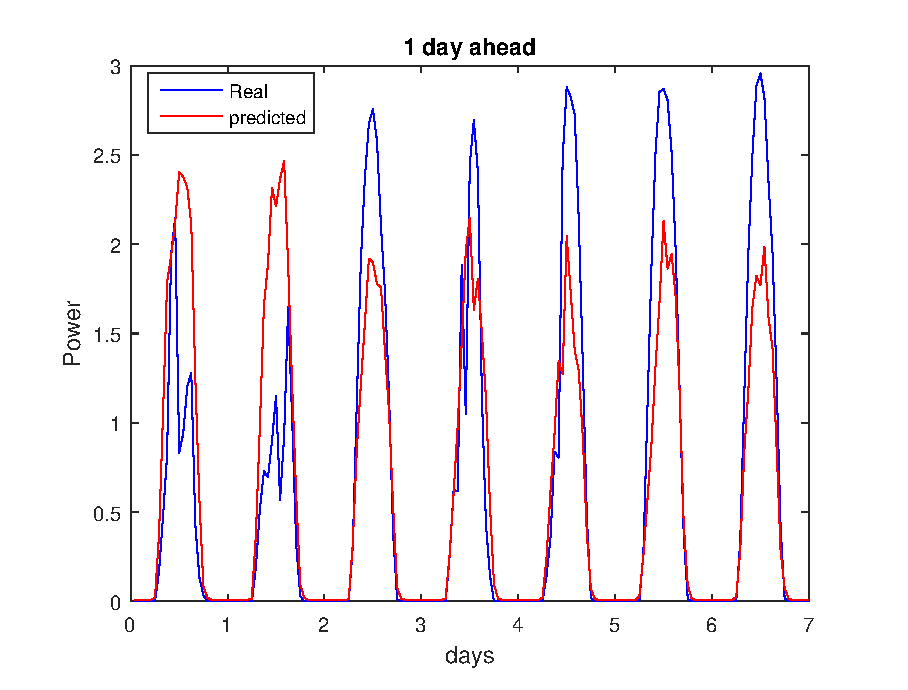
\includegraphics[width=.3\linewidth]{figs/solar_ar_1_day_ahead}}
%	\subfloat[Wind Generation]{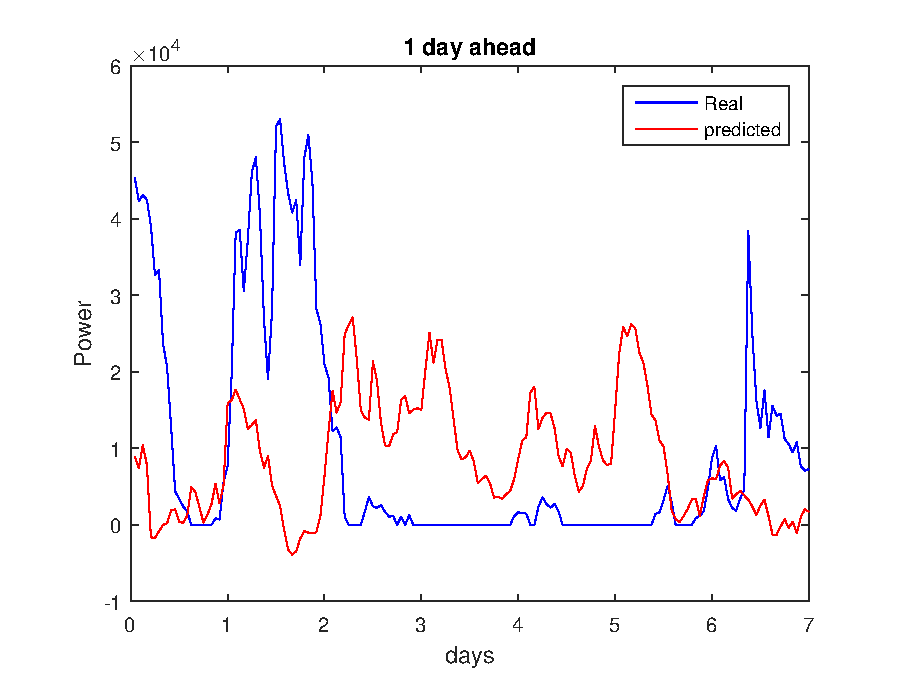
\includegraphics[width=.3\linewidth]{figs/wind_ar_1_day_ahead}}
%	\subfloat[Price          ]{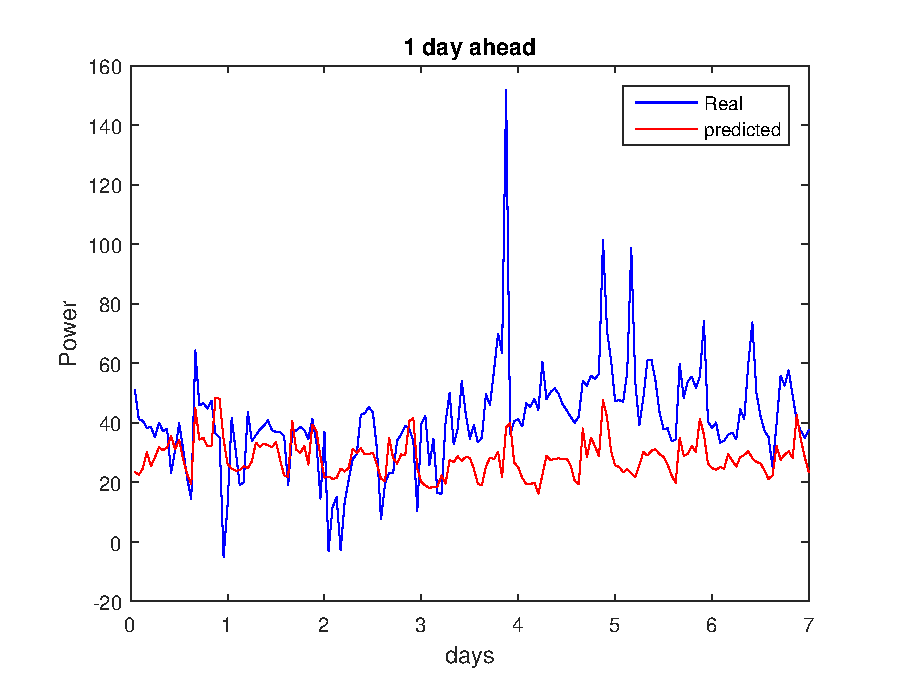
\includegraphics[width=.3\linewidth]{figs/price_ar_1_day_ahead}}
%	%\subfloat[Workload       ]{\includegraphics[width=.2\linewidth]{figs/rosette}}
%	\caption{1 day ahead AR prediction of PV generation (a), Wind generation (b), Electricity prices (c), and workload (d).}
%	\label{fig:periodgram}
%\end{figure*}

%\begin{figure*}[!h]
%	\centering
%	\subfloat[PV Generation  ]{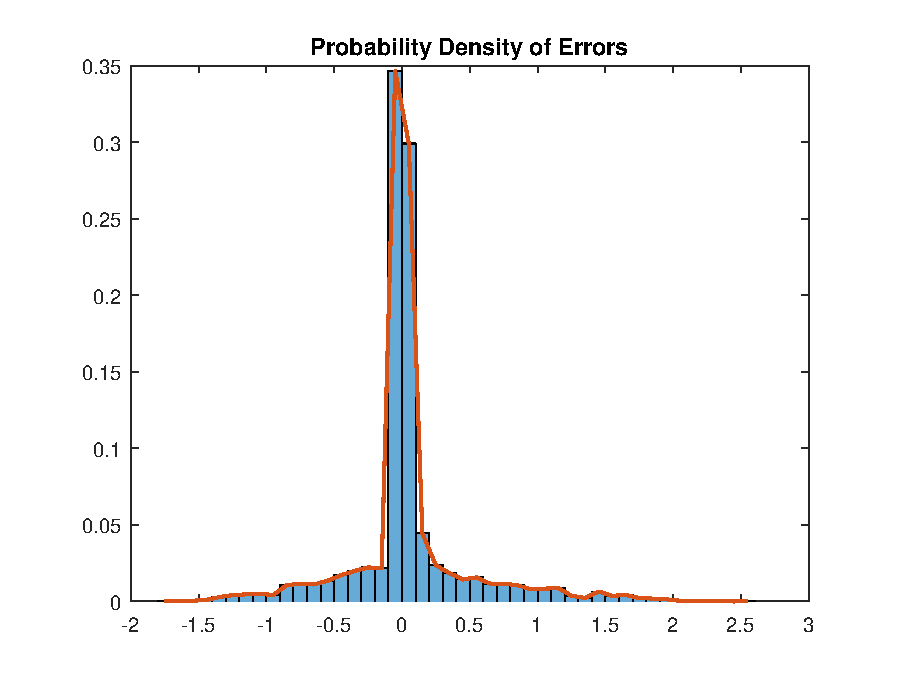
\includegraphics[width=.3\linewidth]{figs/solar_ar_1_day_ahead_pdf}}
%	\subfloat[Wind Generation]{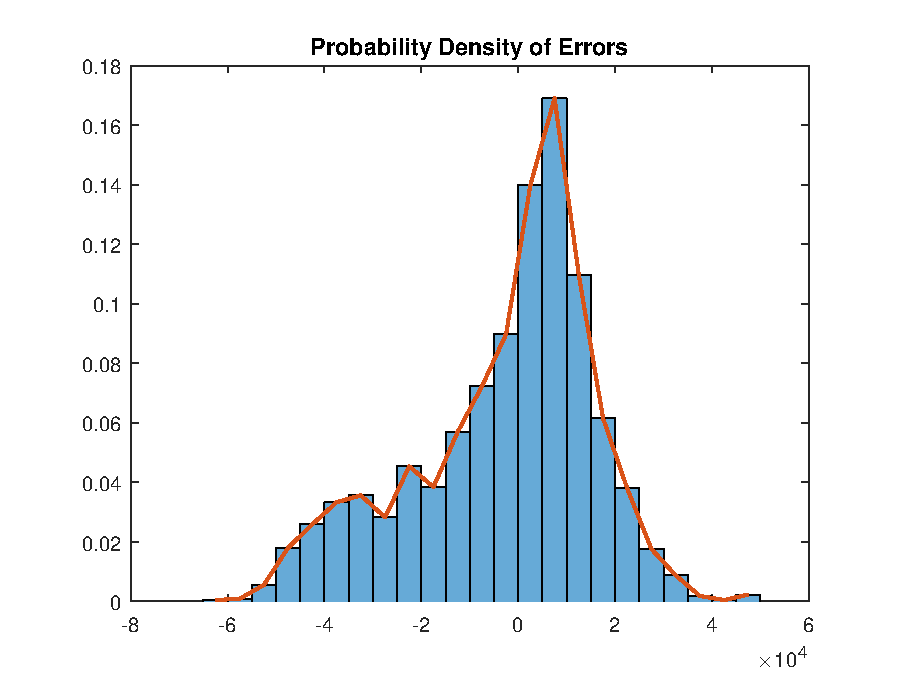
\includegraphics[width=.3\linewidth]{figs/wind_ar_1_day_ahead_pdf}}
%	\subfloat[Price          ]{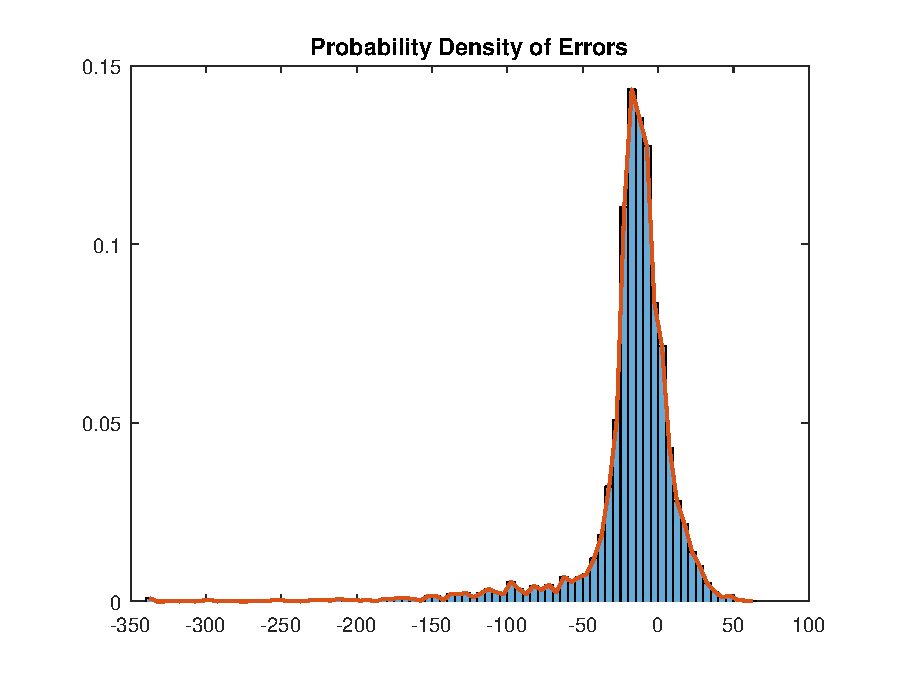
\includegraphics[width=.3\linewidth]{figs/price_ar_1_day_ahead_pdf}}
%	%\subfloat[Workload       ]{\includegraphics[width=.2\linewidth]{figs/rosette}}
%	\caption{pdf(probability desity function) of 1 day ahead AR prediction errors for PV generation (a), Wind generation (b), Electricity prices (c), and workload (d).}
%	\label{fig:periodgram}
%\end{figure*}
%
%\begin{figure*}[!h]
%	\centering
%	\subfloat[PV Generation  ]{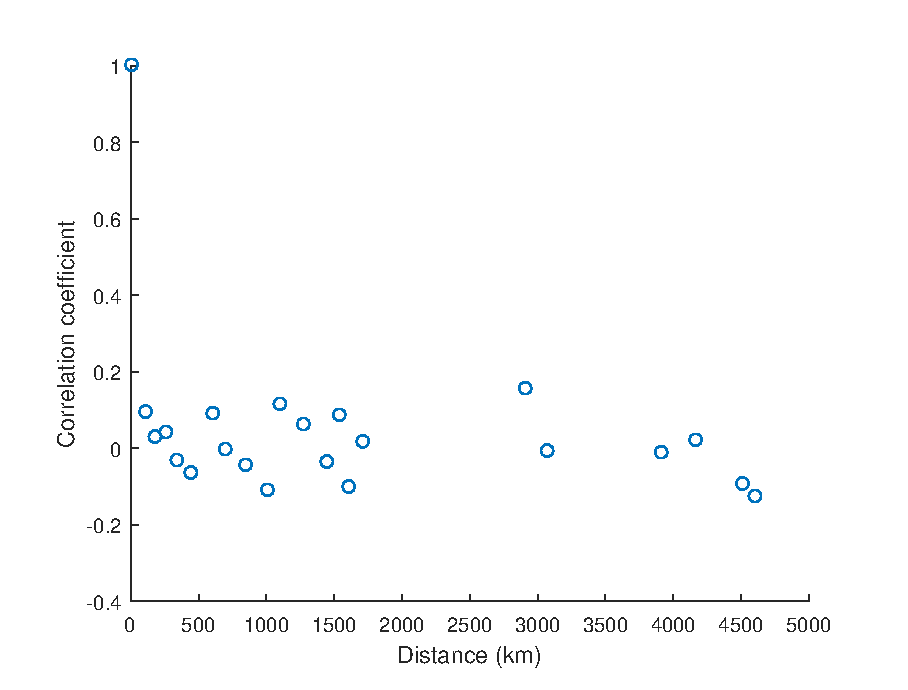
\includegraphics[width=.3\linewidth]{figs/solar_ar_corr_coff_1}}
%	\subfloat[Wind Generation]{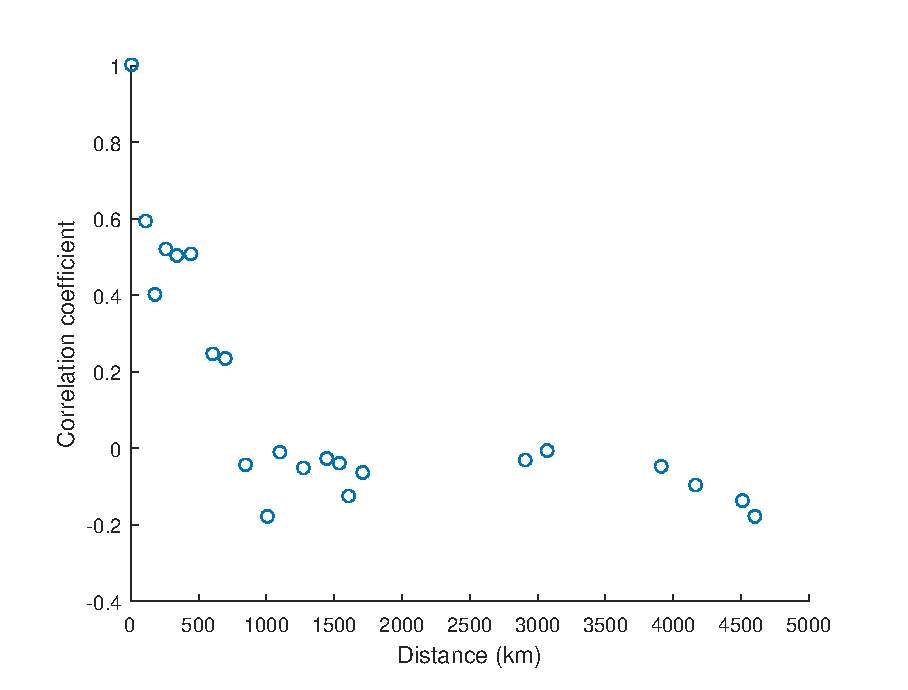
\includegraphics[width=.3\linewidth]{figs/wind_ar_corr_coff_1}}
%	%\subfloat[Price          ]{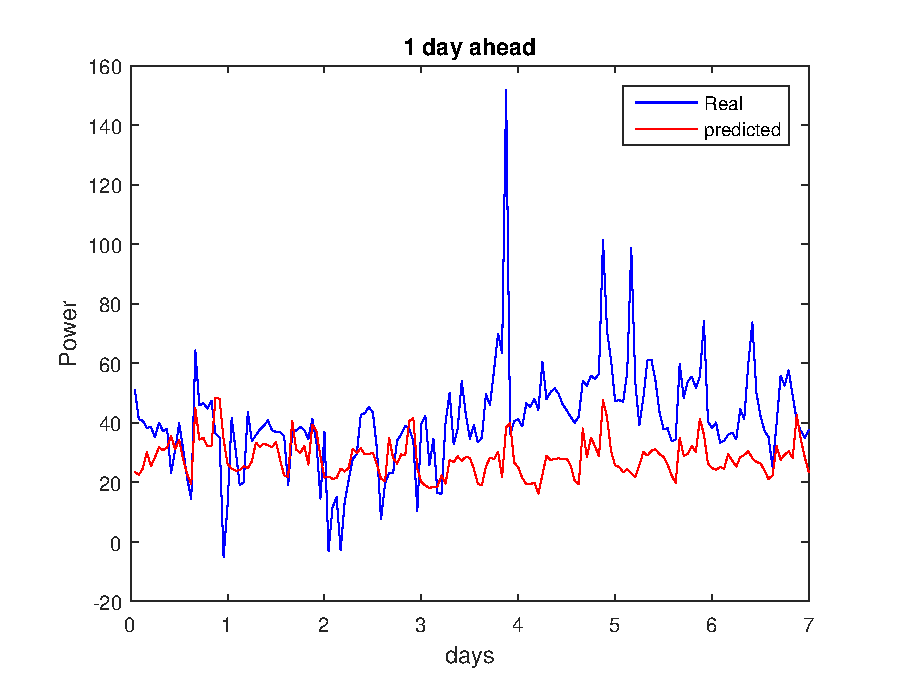
\includegraphics[width=.2\linewidth]{figs/price_ar_1_day_ahead}}
%	%\subfloat[Workload       ]{\includegraphics[width=.2\linewidth]{figs/rosette}}
%	\caption{Correlation Cofficients in space domain for 1 day ahead AR prediction of PV generation (a), Wind generation (b), Electricity prices (c), and workload (d).}
%	\label{fig:periodgram}
%\end{figure*}

%\begin{figure}[!h]
%	\centering
%	\subfloat[PV Generation  ]{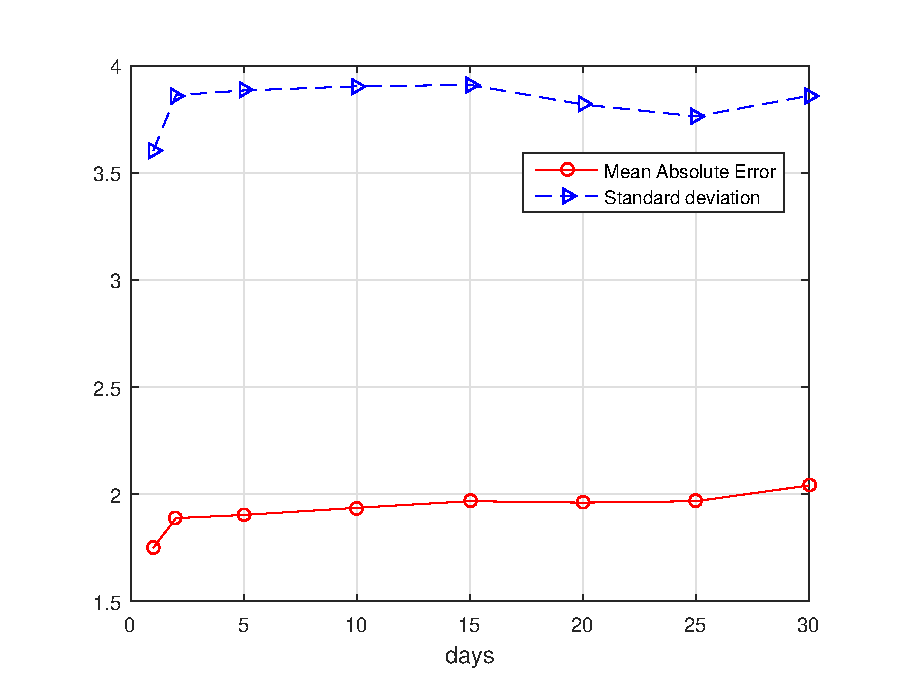
\includegraphics[width=.5\linewidth]{figs/mean_abs_error}}
%	\subfloat[Prices         ]{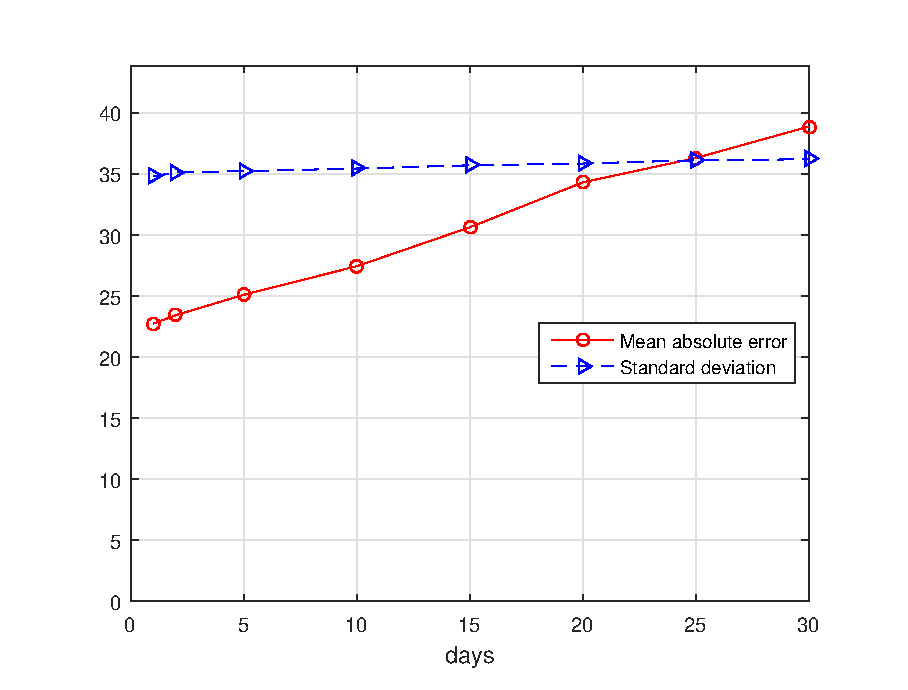
\includegraphics[width=.5\linewidth]{figs/price_mean_absolute_error}}
%	\caption{Mean absolute and standard deviation of prediction error using AR method.(a) PV Generation (b) Prices}
%	\label{fig:periodgram}
%\end{figure}

%\desc{Average of the past 60 days.}

%\begin{figure*}[!h]
%	\centering
%	\subfloat[PV Generation  ]{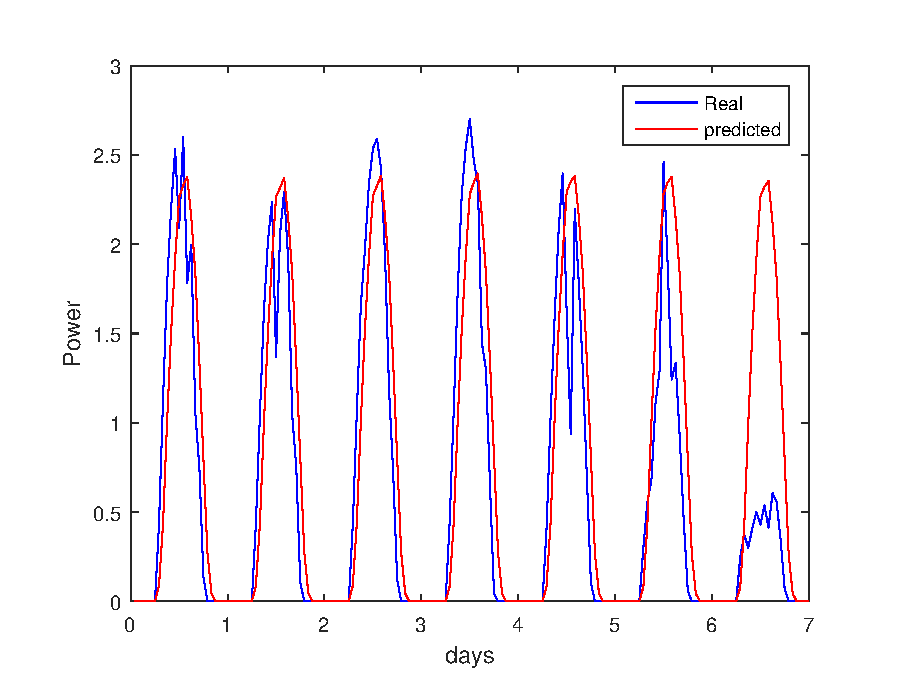
\includegraphics[width=.3\linewidth]{figs/solar_avg}}
%	\subfloat[Wind Generation]{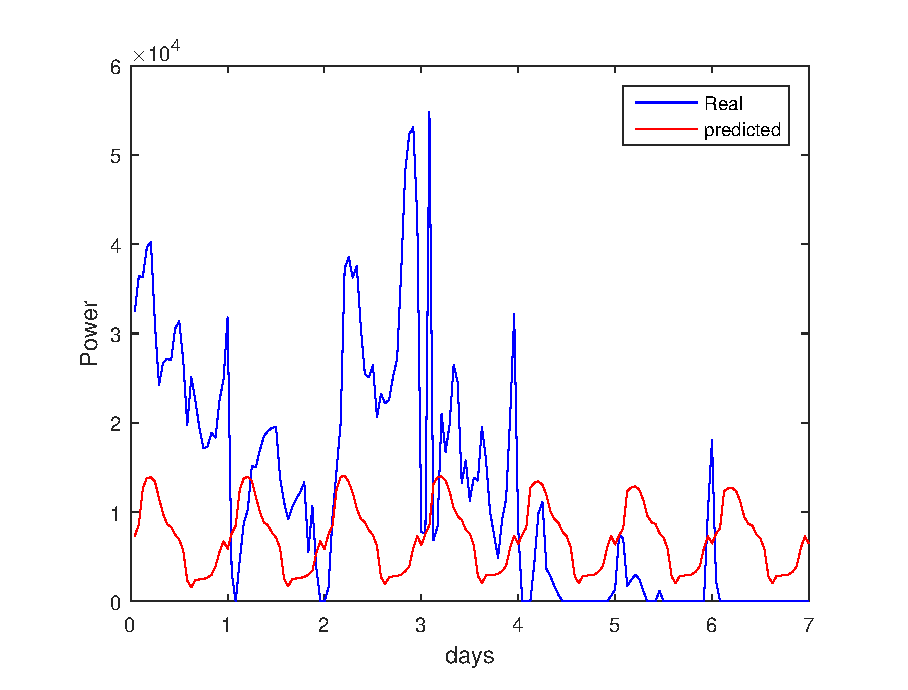
\includegraphics[width=.3\linewidth]{figs/wind_avg}}
%	\subfloat[Price          ]{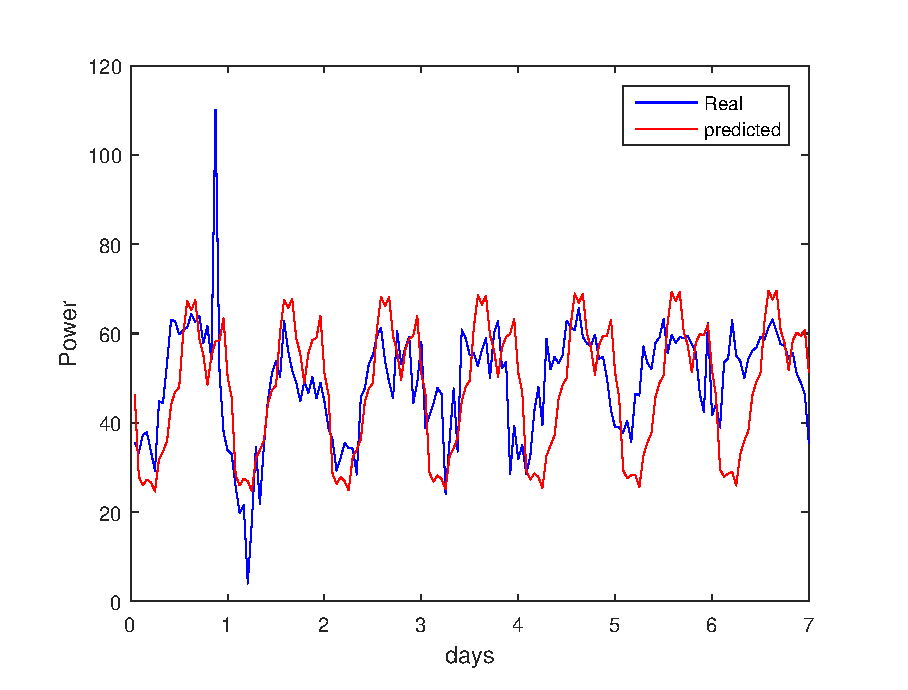
\includegraphics[width=.3\linewidth]{figs/price_avg}}
%	%\subfloat[Workload       ]{\includegraphics[width=.2\linewidth]{figs/rosette}}
%	\caption{Averaging past 60 days to predict PV generation (a), Wind generation (b), Electricity prices (c), and workload (d).}
%	\label{fig:periodgram}
%\end{figure*}
%
%\begin{figure*}[!h]
%	\centering
%	\subfloat[PV Generation  ]{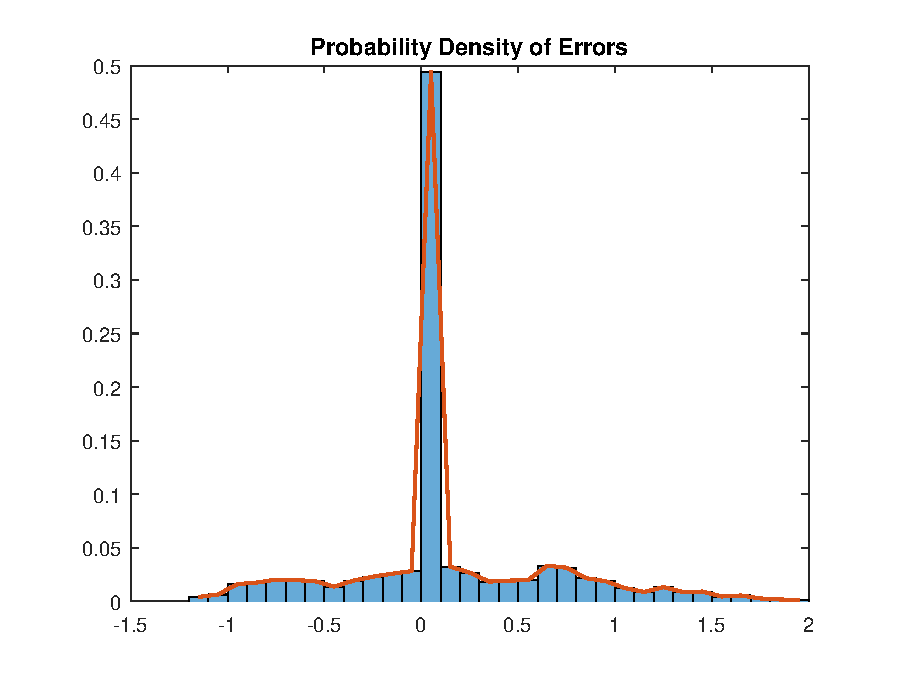
\includegraphics[width=.3\linewidth]{figs/solar_avg_pdf}}
%	\subfloat[Wind Generation]{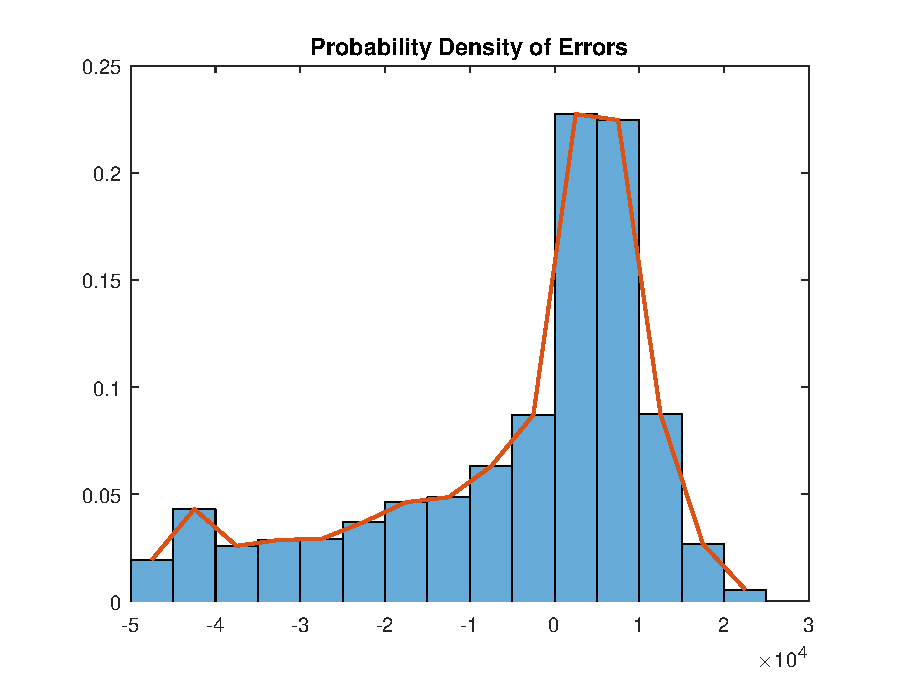
\includegraphics[width=.3\linewidth]{figs/wind_avg_pdf}}
%	\subfloat[Price          ]{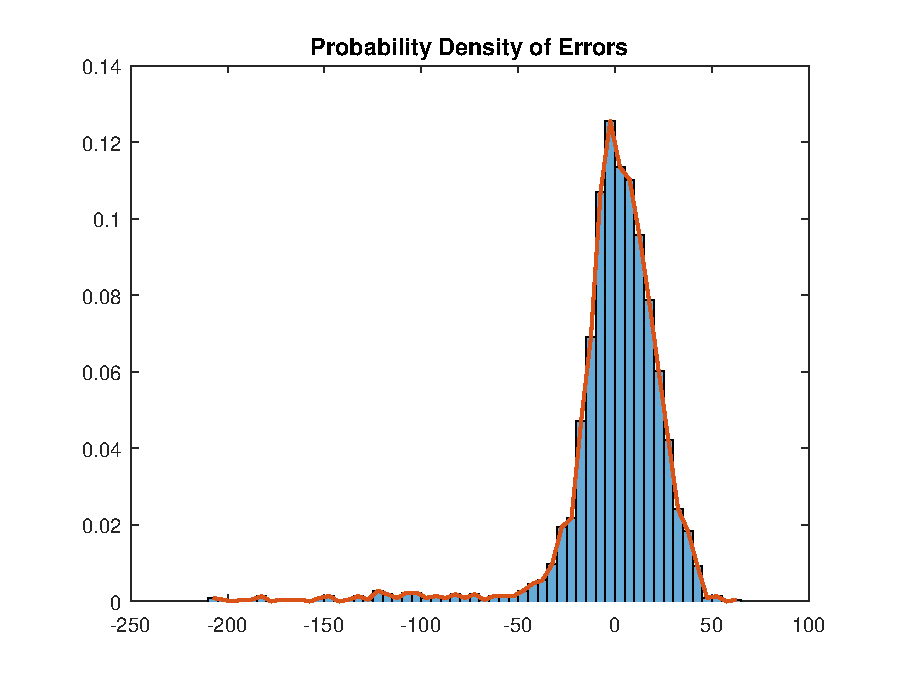
\includegraphics[width=.3\linewidth]{figs/price_avg_pdf}}
%	%\subfloat[Workload       ]{\includegraphics[width=.2\linewidth]{figs/rosette}}
%	\caption{pdf(probability desity function) of averaging prediction errors for PV generation (a), Wind generation (b), Electricity prices (c), and workload (d).}
%	\label{fig:periodgram}
%\end{figure*}
%
%\begin{figure*}[!h]
%	\centering
%	\subfloat[PV Generation  ]{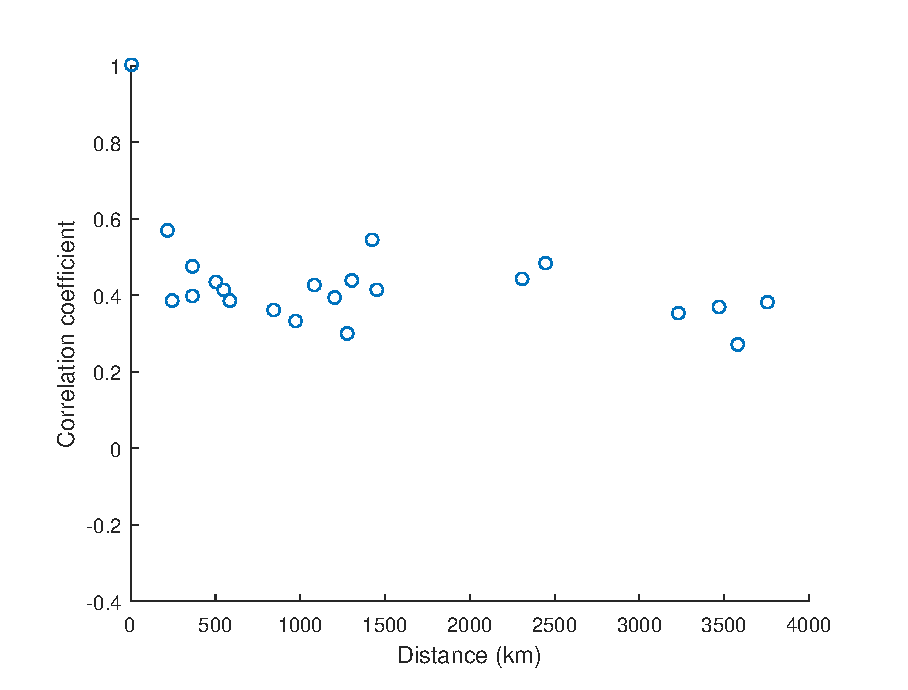
\includegraphics[width=.3\linewidth]{figs/solar_avg_corr_coff}}
%	\subfloat[Wind Generation]{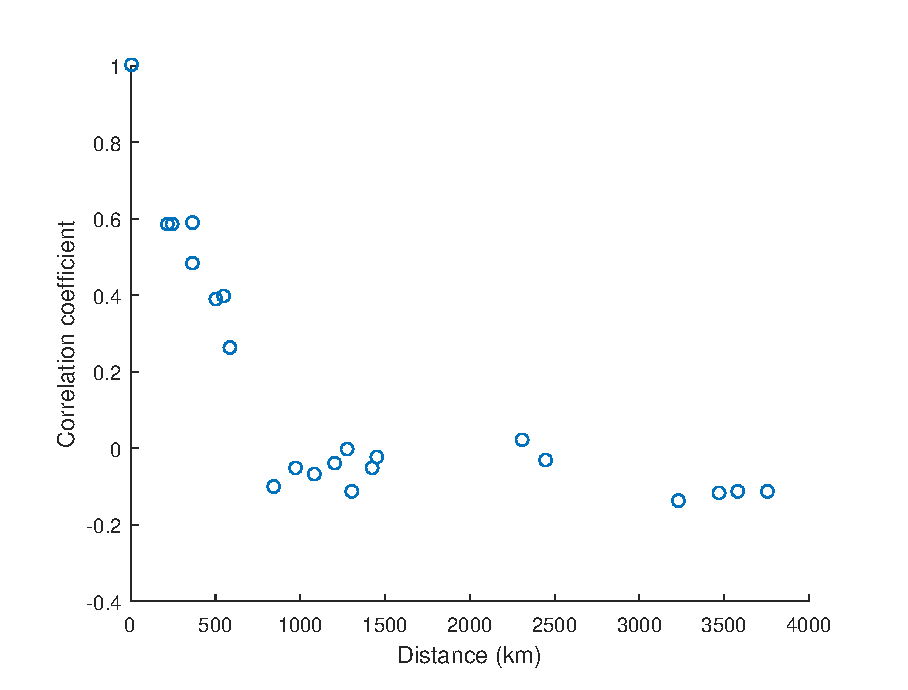
\includegraphics[width=.3\linewidth]{figs/wind_avg_corr_coff}}
%	%\subfloat[Price          ]{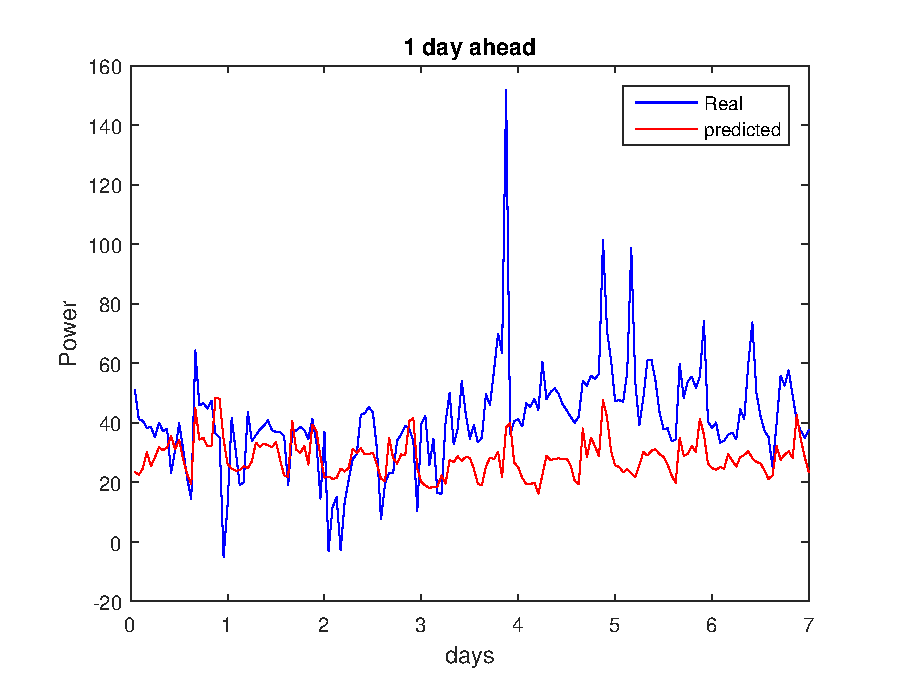
\includegraphics[width=.2\linewidth]{figs/price_ar_1_day_ahead}}
%	%\subfloat[Workload       ]{\includegraphics[width=.2\linewidth]{figs/rosette}}
%	\caption{Correlation Cofficients in space domain for averaging prediction errors of PV generation (a), Wind generation (b), Electricity prices (c), and workload (d).}
%	\label{fig:periodgram}
%\end{figure*}



%We implement SVM (Support Vector Machine) method to predict the PV generation and wind generation in long term. We assume that we can obtain the forecast conditions from trusted sources for example, weather forecast services. The input parameters for predicting PV generation are hour of day, ambient temperature, angle of incidence, sun up over horizon, dry bulk temperature, wet bulk temperature, dew point temperature, relative humidity, wind speed and wind direction. The input parameters for wind generation forecast are wind speed, wind direction, air temperature, and pressure.

%\begin{figure*}[!h]
%	\centering
%	\subfloat[PV Generation  ]{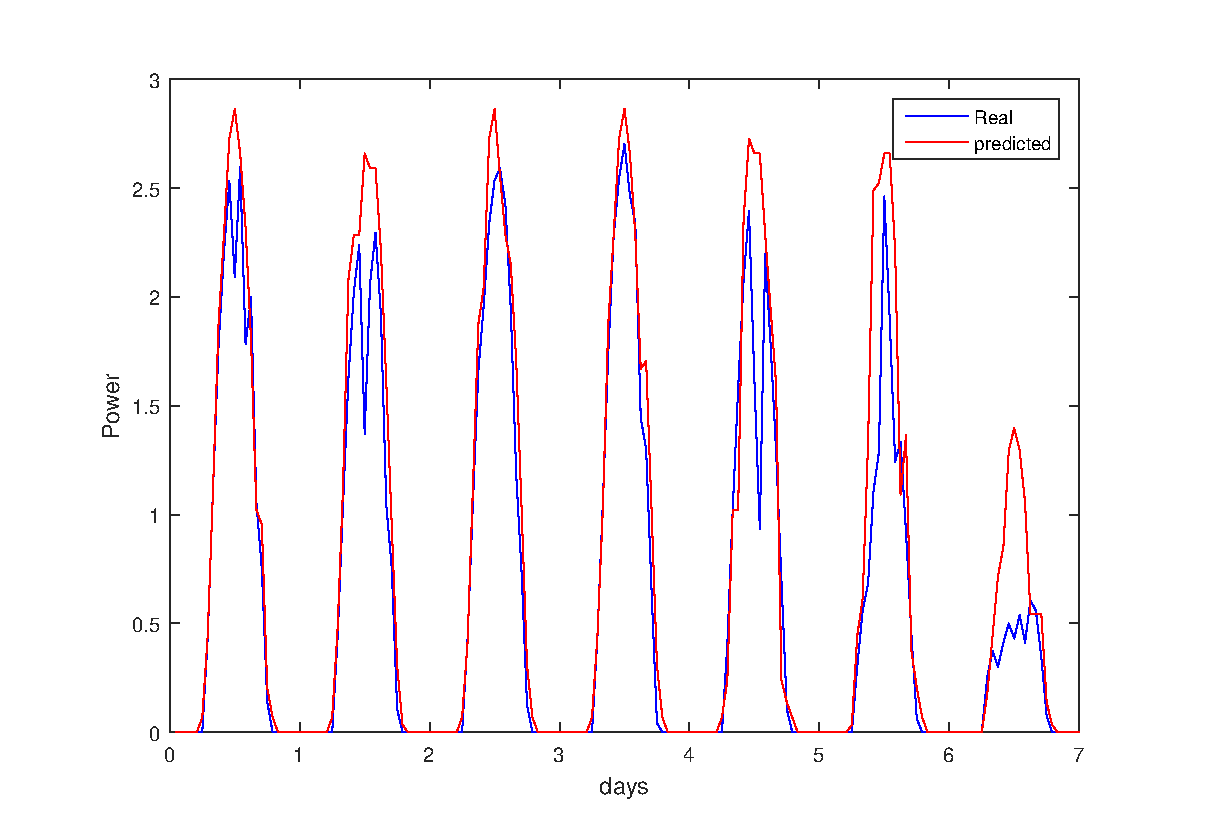
\includegraphics[width=.3\linewidth]{figs/solar_svm}}
%	\subfloat[Wind Generation]{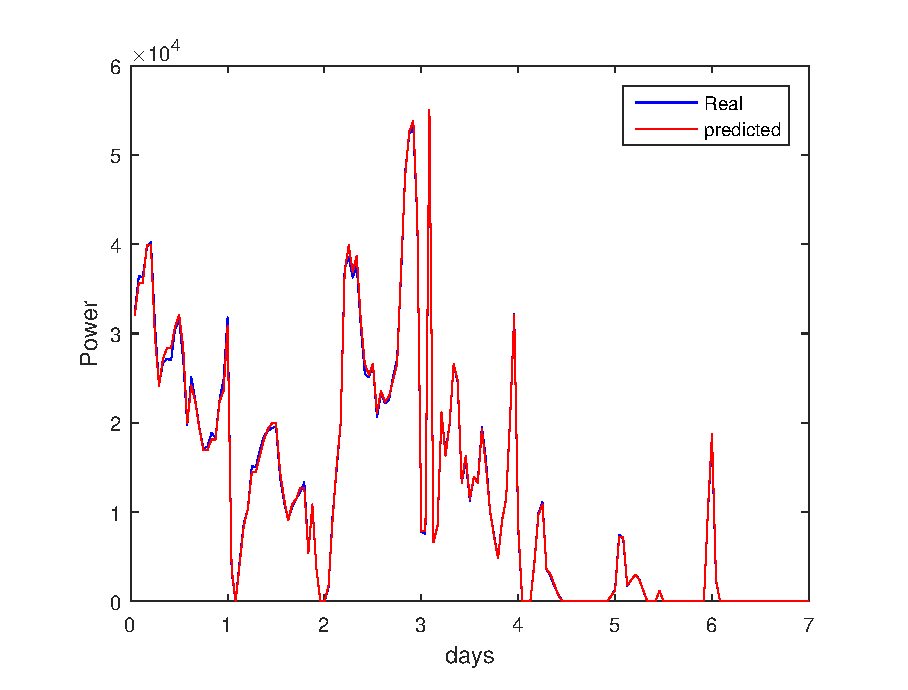
\includegraphics[width=.3\linewidth]{figs/wind_svm}}
%	%\subfloat[Price          ]{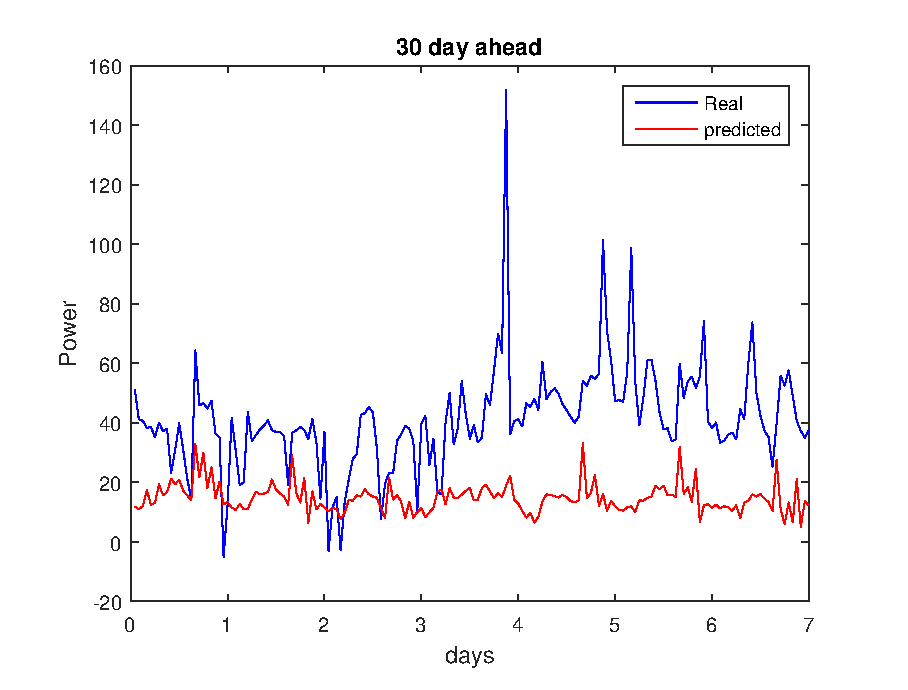
\includegraphics[width=.2\linewidth]{figs/price_ar_30_day_ahead}}
%	%\subfloat[Workload       ]{\includegraphics[width=.2\linewidth]{figs/rosette}}
%	\caption{SVM prediction of PV generation (a) PV generation, Wind generation (b), Electricity prices (c), and workload (d).}
%	\label{fig:periodgram}
%\end{figure*}
%
%\begin{figure*}[!h]
%	\centering
%	\subfloat[PV Generation  ]{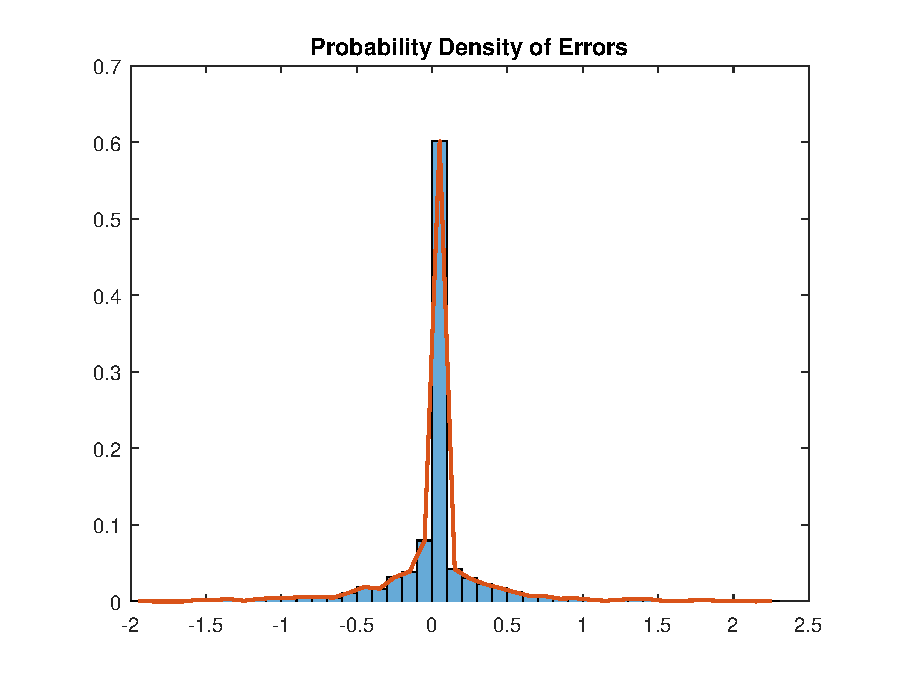
\includegraphics[width=.3\linewidth]{figs/solar_svm_pdf}}
%	\subfloat[Wind Generation]{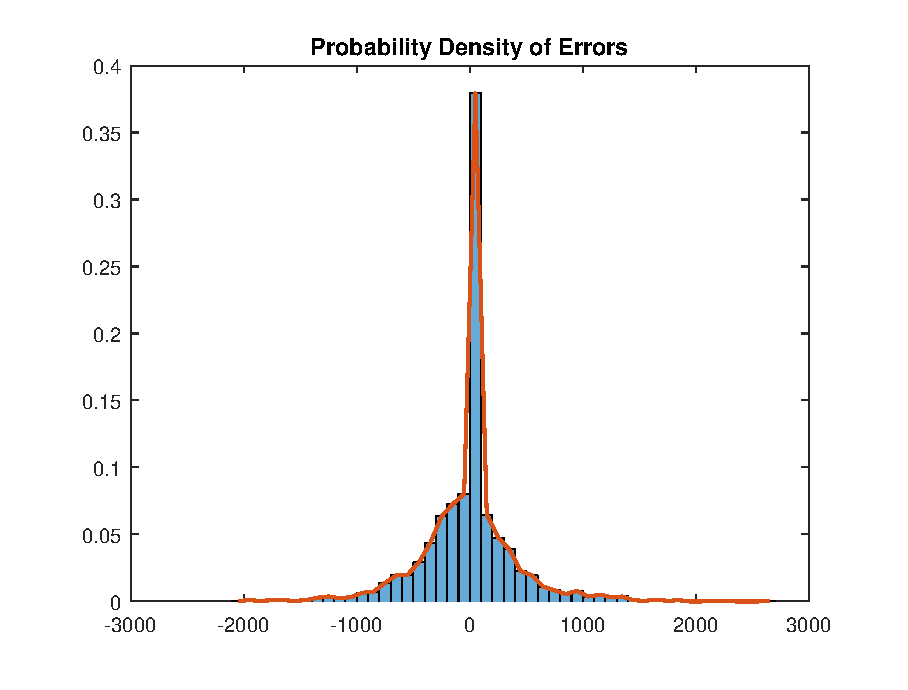
\includegraphics[width=.3\linewidth]{figs/wind_svm_pdf}}
%	%\subfloat[Price          ]{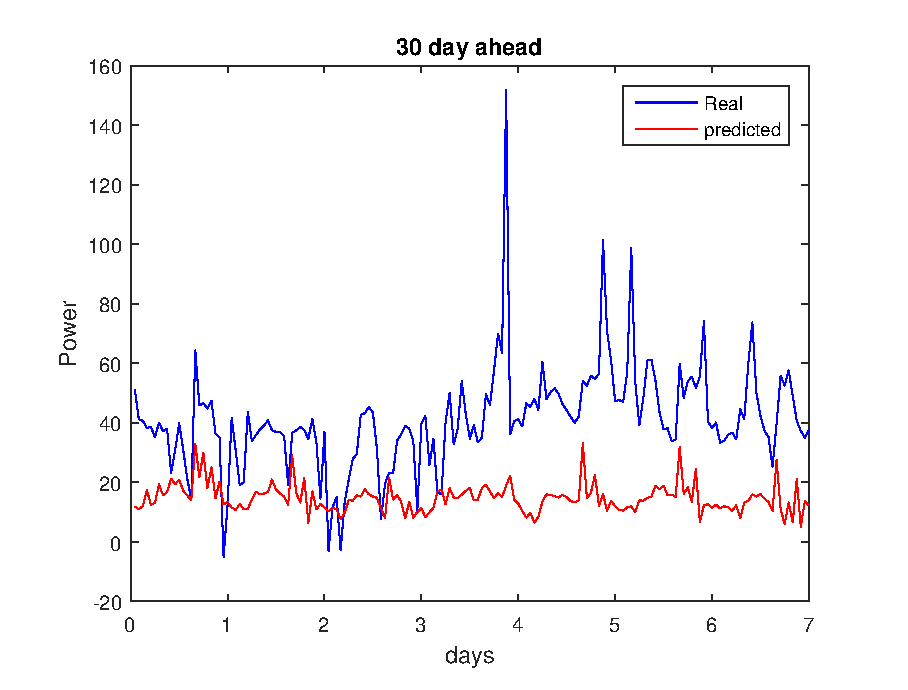
\includegraphics[width=.2\linewidth]{figs/price_ar_30_day_ahead}}
%	%\subfloat[Workload       ]{\includegraphics[width=.2\linewidth]{figs/rosette}}
%	\caption{pdf of SVM prediction errors for PV generation (a), Wind generation (b), Electricity prices (c), and workload (d).}
%	\label{fig:periodgram}
%\end{figure*}
%
%
%\begin{figure*}[!h]
%	\centering
%	\subfloat[PV Generation  ]{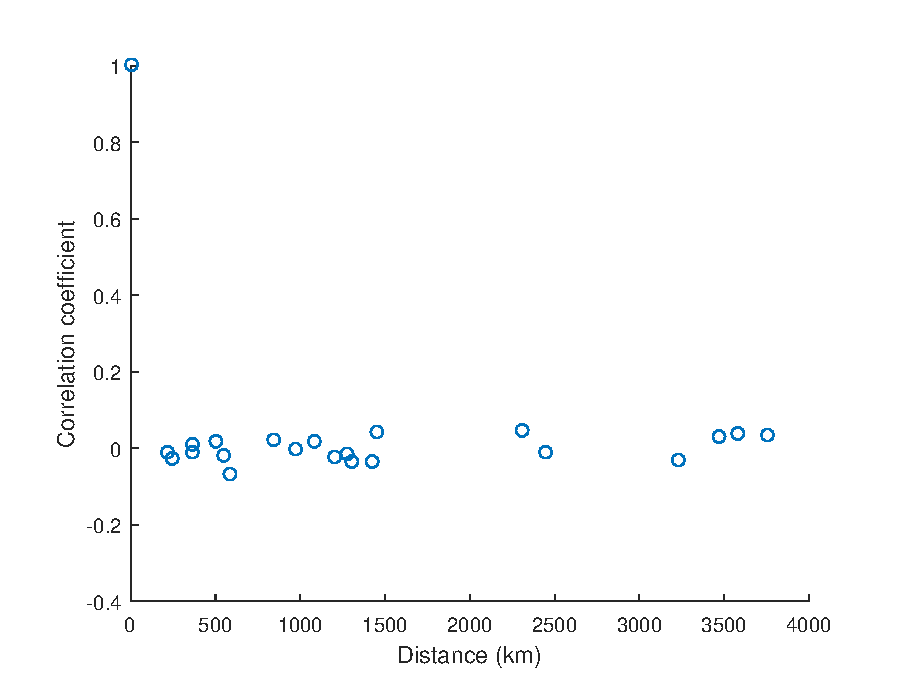
\includegraphics[width=.3\linewidth]{figs/solar_svm_corr_coff}}
%	\subfloat[Wind Generation]{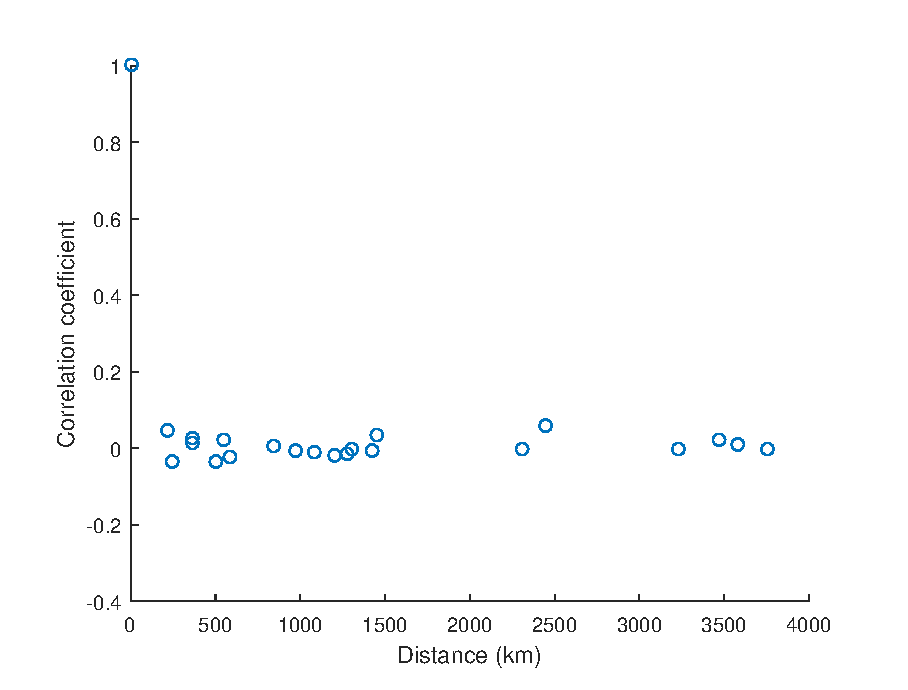
\includegraphics[width=.3\linewidth]{figs/wind_svm_corr_coff}}
%	%\subfloat[Price          ]{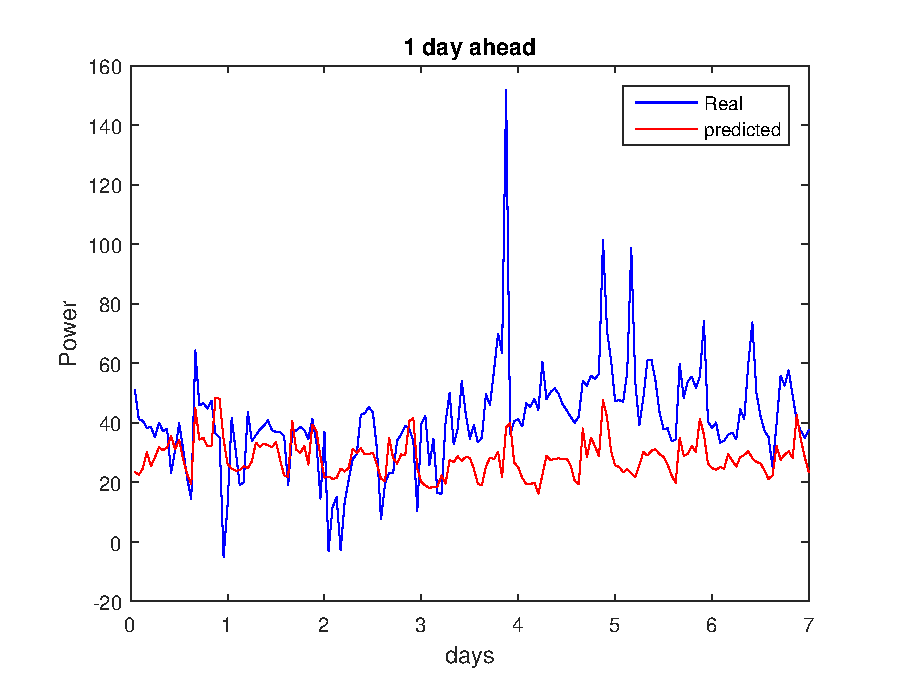
\includegraphics[width=.25\linewidth]{figs/price_ar_1_day_ahead}}
%	%\subfloat[Workload       ]{\includegraphics[width=.25\linewidth]{figs/rosette}}
%	\caption{Correlation Cofficients in space domain for SVM prediction of PV generation (a), Wind generation (b), Electricity prices (c), and workload (d).}
%	\label{fig:periodgram}
%\end{figure*}
%
%\begin{figure*}[!h]
%	\centering
%	%\subfloat[AR 1 hour ahead ]{\includegraphics[width=.25\linewidth]{figs/corr_coff_solar_wind_ar_adv}}
%	\subfloat[AR 1 day ahead  ]{\includegraphics[width=.25\linewidth]{figs/corr_coff_solar_wind_ar_1}}
%	\subfloat[AR 30 day ahead ]{\includegraphics[width=.25\linewidth]{figs/corr_coff_solar_wind_ar_30}}
%	\subfloat[SVM             ]{\includegraphics[width=.25\linewidth]{figs/corr_coff_solar_wind_svm}}
%	\caption{Cross Correlation Cofficients of prediction errors between PV vs. Wind generation in different locations (a) AR 1 day ahead (b) AR 30 day ahead (c) SVM.}
%	\label{fig:periodgram}
%\end{figure*}


%http://forecast.weather.gov/MapClick.php?w0=t&w1=td&w2=wc&w3=sfcwind&w3u=1&w4=sky&w5=pop&w6=rh&w7=rain&w8=thunder&w9=snow&w10=fzg&w11=sleet&w13u=0&w16u=1&AheadHour=96&FcstType=graphical&textField1=43.0798&textField2=-89.3875&site=all&unit=0&dd=&bw=&BackDay.x=66&BackDay.y=9&BackDay=48


%Forward electricity markets have been proposed with real-time (spot) electricity markets to improve the design of electricity markets. Forward electricity markets have been adopted in Colombia in 2008 \cite{cramton2007colombia}. The forward markets include both long term (several months) and short term (day-ahead). Via the long term contract between supply and demand, the electricity use is adequate for customers. The forward electricity markets reduce of the risk both side of supply and demand since they reduce the quantity of energy trading at real-time \cite{ausubel2010using}. Furthermore, purchasing electricity ahead contribute to the expansion of renewable energy sources (RESs). For example, Google invest in purchasing renewable energy from renewable project developers for 20 years \cite{google2015datacenter}. 

%The uncertainties of workload demand, renewable energy, and electricity prices at real time are the most challenges for data centers in the long term markets. The workload demand from cloud users and renewable energy generation are uncontrollable, and intermittent \cite{gan2013real, liu2012renewable}. The volatility of electricity prices also introduce financial risk in real time markets \cite{liu2013applying}. The uncertainties may cause the significant risk for data centers if data center operators under or over procure the power in the long term due to their huge consumption.

%\begin{figure*}[!h]
%	\centering
%	\subfloat[PV Generation  ]{\includegraphics[width=.3\linewidth]{figs/solar_ar_30_day_ahead}}
%	\subfloat[Wind Generation]{\includegraphics[width=.3\linewidth]{figs/wind_ar_30_day_ahead}}
%	%	\subfloat[Price          ]{\includegraphics[width=.3\linewidth]{figs/price_ar_30_day_ahead}}
%	%\subfloat[Workload       ]{\includegraphics[width=.2\linewidth]{figs/rosette}}
%	\caption{30 day ahead AR prediction of PV generation (a), Wind generation (b), Electricity prices (c), and workload (d).}
%\end{figure*}

%\begin{figure*}[!ht]
%	\centering
%	\subfloat[PV Generation  ]{\includegraphics[width=.5\linewidth]{figs/solar_autocorrelation}}
%	\subfloat[Wind Generation]{\includegraphics[width=.5\linewidth]{figs/wind_autocorrelation}}
%%	\subfloat[Price          ]{\includegraphics[width=.3\linewidth]{figs/price_autocorr}}
%	%\subfloat[Workload       ]{\includegraphics[width=.2\linewidth]{figs/rosette}}
%	\caption{The auto-correlation of PV generation (a), Wind generation (b), Electricity prices (c), and workload (d).}
%	\label{fig:auto-correlation}
%\end{figure*}


%\begin{figure*}[!h]
%	\centering
%	\subfloat[PV Generation  ]{\includegraphics[width=.3\linewidth]{figs/solar_ar_30_day_ahead}}
%	\subfloat[Wind Generation]{\includegraphics[width=.3\linewidth]{figs/wind_ar_30_day_ahead}}
%	%	\subfloat[Price          ]{\includegraphics[width=.3\linewidth]{figs/price_ar_30_day_ahead}}
%	%\subfloat[Workload       ]{\includegraphics[width=.2\linewidth]{figs/rosette}}
%	\caption{30 day ahead AR prediction of PV generation (a), Wind generation (b), Electricity prices (c), and workload (d).}
%\end{figure*}

%\begin{figure}[!h]
%	\centering
%	\subfloat[PV Generation  ]{\includegraphics[width=.5\linewidth]{figs/solar_ar_30_day_ahead_pdf}}
%	\subfloat[Wind Generation]{\includegraphics[width=.5\linewidth]{figs/wind_ar_30_day_ahead_pdf}}
%	%	\subfloat[Price          ]{\includegraphics[width=.3\linewidth]{figs/price_ar_30_day_ahead_pdf}}
%	%\subfloat[Workload       ]{\includegraphics[width=.2\linewidth]{figs/rosette}}
%	\caption{pdf(probability desity function) of 30 day ahead AR prediction errors for PV generation (a), Wind generation (b), Electricity prices (c), and workload (d).}
%\end{figure}

%\begin{figure}[!h]
%	\centering
%	\subfloat[PV Generation  ]{\includegraphics[width=.5\linewidth]{figs/solar_ar_autocoff_30}}
%	\subfloat[Wind Generation]{\includegraphics[width=.5\linewidth]{figs/wind_ar_autocoff_30}}
%	%\subfloat[Price          ]{\includegraphics[width=.2\linewidth]{figs/price_ar_1_day_ahead}}
%	%\subfloat[Workload       ]{\includegraphics[width=.2\linewidth]{figs/rosette}}
%	\caption{Autocorrelation of 30 day ahead AR prediction errors of PV generation (a), Wind generation (b), Electricity prices (c), and workload (d).}
%\end{figure}



\subsection{Proof of Theorem \ref{theorem:ZeroProcurementInLongTerm}}
\label{proof:ZeroProcurementInLongTerm}

Assume that the optimal solution $S$ has $q^{l}_k > 0$ at data center $i$ with $p^l_k \geq \mathbb{E}[p^r_k]$. The idea is to show that there exists a better solution $S'$ with $q^{l}_k{'} = 0$. 

We choose the solution $S$ such that all $q^l_i$, $m_i$, and $\lambda_{ij}$ are equivalent to $S$ except $q^{l}_k{'} = 0$. 
The expected cost of $S$ and $S'$ are respectively $\text{EC}(S)$ and $\text{EC}(S')$. We prove that 
\begin{eqnarray}
\text{EC}(S') \leq \text{EC}(S)
\end{eqnarray}
Expanding $\text{EC}(S)$ and $\text{EC}(S')$ from \eqref{eq:expectedCost}, we have the following inequality
\begin{align}
	\mathbb{E}[p^r_k [m_k - 0 - w^r_k]_+] \leq p^l_k q^l_k + \mathbb{E}[[p^r_k m_k - q^l_k - w^r_k]_+]
\end{align}
We consider the 2 following cases of $m_k$,
\begin{enumerate}
	\item When $m_k \geq q^l_k+w^r_k$, the inequality becomes
	\begin{align}
		&	\mathbb{E}[p^r_k m_k] - \mathbb{E}[p^r_k w^r_k] \leq p^l_k q^l_k + \mathbb{E}[p^r_k m_k] -\mathbb{E}[p^r_k]q^l_k - \mathbb{E}[p^r_k w^r_k] \\
		&\Leftrightarrow	0 \leq p^l_k q^l_k  -\mathbb{E}[p^r_k]q^l_k \\
		&\Leftrightarrow	\mathbb{E}[p^r_k]  \leq p^l_k 
	\end{align}	
	\item 	When $m_k < q^l_k+w^r_k$, the inequality becomes
	\begin{align}
		\mathbb{E}[p^r_k [m_k - w^r_k]_+] < p^l_k q^l_k
	\end{align}
	We have $[m_k- w^r_k]_+ \leq q^l_k$ because $m_k- w^r_k<q^l_k$ and $q^l_k > 0$. Hence,
	\begin{align}
		\mathbb{E}[p^r_k [m_k - w^r_k]_+] < \mathbb{E}[p^r_k] q^l_k \leq p^l_k q^l_k
	\end{align}		
\end{enumerate}
So, the inequality holds which indicates that $q^l_k=0$ when $p^l_k \geq \mathbb{E}[p^r_k]$.

\subsection{Optimality conditions} Let $L$ is the Lagrangian of GLB-RT

\begin{align}
	L = \sum_{i=1}^{N} p^r_i q^r_i + \sum_{i}^{}\sum_{j}^{}h_{ij}(m_i, \lambda_{ij}) \nonumber \\
	- \sum_{i}^{}\sum_{j}^{} \delta_{ij} \lambda_{ij}  + \sum_{j}^{}\upsilon_j(L^r_j - \sum_{j=1}^{J} \lambda_{ij})  \nonumber \\
	+ \sum_{i}^{}(\bar{\omega}_i(m_i-M_i) - \underbar{$\omega$}_i m_i) + \sum_{i} \sigma_i (m_i\mu_i - \lambda_i) \nonumber \\
	- \sum_{i}^{}\kappa_i q^r_i + \sum_{i}^{}\varrho_i(-q^r_i + m_i - w^r_i - q^l_i) 
\end{align}
where $\delta_{ij}, \upsilon_j, \bar{\omega}_i, \underbar{$\omega$}_i, \sigma_i, \kappa_i, \varrho_i$ are Langrange multipliers.  The stationary, complementary slackness, primal feasibility, and dual feasibility of KKT conditions are as follows.
\begin{eqnarray}
\label{eq:KKTStationary1}
\beta (\frac{\mu_i}{(\mu_i-\frac{\lambda_i}{m_i})^2}+\pi_{ij}) - \upsilon_j - \delta_{ij} -\sigma_i = 0 \\
\delta_{ij}\lambda_{ij} = 0; \delta_{ij} \geq 0, \lambda_{ij} \geq 0, \\
\label{eq:FeasiblityLambda1}
\sigma_i(m_i\mu_i-\lambda_i) = 0; \sigma_i \geq 0, m_i\mu_i - \lambda_i \geq 0, \\
\label{eq:FeasiblityLambda2}
\sum_{i}^{}	\lambda_{ij} = L^r_j \\
\label{eq:KKTStationary2}
- \beta \bigg (\frac{\frac{\lambda_i}{m_i}}{\mu_i - \frac{\lambda_i}{m_i}}\bigg)^2 + \bar{\omega}_i - \underbar{$\omega$}_i + \sigma_i\mu_i + \varrho_i = 0 \\
\bar{\omega}_i(m_i - M_i) = 0; \bar{\omega}_i \geq 0, m_i \leq M_i \\
\label{eq:KKTStationary2_1}
\underbar{$\omega$}_i m_i = 0; \underbar{$\omega$}_i \geq 0, m_i \geq 0 \\
\label{eq:KKTStationary3}
p_i^r - \kappa_i - \varrho_i = 0 \\
\label{eq:Feasiblity_q}
\kappa_i q^r_i = 0; \kappa_i \geq 0, q^r_i \geq 0 \\
\varrho_i(-q^r_i + m_i - w^r_i - q^l_i)  = 0; \nonumber \\ \varrho_i \geq 0, q^r_i \geq m_i - w^r_i - q^l_i 
\end{eqnarray}
Let us call $\bar{\lambda}_i = \lambda_i/m_i$ the server arrival rate.

$m_i=0$ is not considered because it makes the term $\lambda_i / m_i$ is not defined in the objective function. It also makes sense because $m_i=0$ is equivalent to shutting down whole data center $i$ can be ignored in our formulation.

We claim that the source $j$ only send data to those data center i which have minimum marginal cost $\pi_{ij} + \frac{(1+\sqrt{p^*_i/\beta})^2}{\mu_i}$. To prove the claim, let $p^*_i = \bar{\omega}_i - \underbar{$\omega$}_i + \varrho_i$. By \eqref{eq:KKTStationary2} and $\sigma_i(m_i\mu_i-\lambda_i) = 0$, we obtain $\frac{\mu_i}{(\mu_i-\bar{\lambda}_i)^2} = \frac{(1+\sqrt{p^*_i / \beta})^2}{\mu_i}$. Substitute the term into \eqref{eq:KKTStationary1},
\begin{eqnarray}
\label{eq:marginalCost}
\pi_{ij} + \frac{(1+\sqrt{p^*_i/\beta})^2}{\mu_i} = \pi_{ij} + \frac{\mu_i}{(\mu_i-\bar{\lambda}_i)^2} = \frac{\upsilon_j+\delta_j}{\beta} \geq \frac{\upsilon_j}{\beta}
\end{eqnarray}
equality happens when $\lambda_{ij} > 0$.

From the above KKT conditions, we also can obtain the relation between $m_i$ and $\lambda_i$ as
\begin{eqnarray}
\label{eq:ServerArrivalRate}
\bar{\lambda}_i = \frac{\lambda_i}{m_i} = \frac{(\mu_i\sqrt{p^*_i/\beta})}{1+\sqrt{p^*_i/\beta}}
\end{eqnarray}
So given $\lambda_i$, $m_i$ can be determined by projecting the solution of $\hat{m}_i = \frac{\lambda_i(1+\sqrt{p^*_i/\beta})}{(\mu_i\sqrt{p^*_i/\beta})}$. From \eqref{eq:KKTStationary1} to \eqref{eq:FeasiblityLambda2}, sources $j$ having given $m_i$ finds $\lambda_{ij}$ depending on $\lambda_{ik}$ where $k \neq j$. Given $m_i$, it is trivial that the data center operator determines $q^r_i$ as
\begin{eqnarray}
q^r_i =  
\begin{cases} 
0  &\mbox{if  } m_i-w^r_i-q^l_i \leq 0 \\ 
m_i-w^r_i+q^l_i & \mbox{if  } m_i-w^r_i-q^l_i > 0. 
\end{cases}
\end{eqnarray}

\subsection{Proof of Theorem \ref{theorem:serverArrivalRate}}
\label{proof:serverArrivalRate}

Consider $m_i = M_i$ for all optimal solutions, and $q^r_i = [M_i-w^r_i-q^l_i]_+$. We assume that there are two optimal solution $S$ and $S'$ with the same $m_i=M_i$ but they have different arrival rates $\lambda_i$ and $\lambda '_i$, respectively. Let $\{s(\lambda_i)\}$ the set of convex combinations of $S$ and $S'$. Since $F_k$ is convex over $m_k$ and $\lambda_k$ for $k \in N$, $F(s(\lambda_i))-F_i(s(\lambda_i))$ is also convex. Furthermore, $F_i$ is strictly convex over $\lambda_i$ that $F(s(\lambda_i))$ is strictly convex over $\lambda_i$. Thus, the optimal $\lambda_i$ is unique.

If $m_i = w^r_i+q^l_i$, the proof is identical to the case of $m_i = M_i$.

If $m_i > w^r_i+q^l_i$, $\bar{\omega}_i = \underbar{$\omega$}_i = \kappa_i=0$ and $\varrho_i = p^r_i$ due to \eqref{eq:KKTStationary3} and \eqref{eq:Feasiblity_q}. As \eqref{eq:ServerArrivalRate}, the server arrival rate is determined by $\bar{\lambda}_i = \frac{\mu_i\sqrt{p^r_i/\beta}}{1+\sqrt{p^r_i/\beta}}$. 

\subsection{Proof of Theorem \ref{theorem:sparsityNJ1}}
\label{proof:sparsityNJ1}

Consider an undirected bipartite graph $G$ with sources and data centers as two independent sets of the graph vertices. So, $G$ has $|J|+|N|$ vertices. If $\lambda_{ij}>0$, we construct an undirected edge between source $j$ and data center $i$. The idea is to show that there exists the acyclic graph $G$ which has at most $|J|+|N|-1$ edges for an optimal solution $S$.

Suppose that $G$ contains a cycle, and $C$ is the minimal cycle, i.e no subset of $C$ is a cycle. Construct a new solution $S(\xi)$ from $S$ by adding $\xi$ to $\lambda_{ij}$ if $(j,i) \in C$, and subtract $\xi$ from $\lambda_{ij}$ if $(j',i) \in C$. By this way, we can remove an edge in cycle $C$ so that $C$ will not be the cycle. We can see the delay cost before and after constructing the new solution $S(\xi)$ as follows.
\begin{eqnarray}
\sum_{(j,i),(j',i) \in C}^{}(h_{ij}(m_i,(\lambda_{ij}+\xi))+h_{ij'}(m_i,(\lambda_{ij'}-\xi))) \\
= \beta \sum_{(j,i),(j',i) \in C}^{}(\lambda_{ij}+\xi)(\frac{1}{\mu_i - \lambda_i/m_i}  + \pi_{ij}) \nonumber \\ 
+(\lambda_{ij'}-\xi)(\frac{1}{\mu_i - \lambda_i/m_i} + \pi_{ij'}) \\
= \beta \sum_{(j,i),(j',i) \in C} \big (\lambda_{ij}(\frac{1}{\mu_i - \lambda_i/m_i}+\pi_{ij})+\xi\pi_{ij} \nonumber \\
+\lambda_{ij'}(\frac{1}{\mu_i - \lambda_i/m_i}+\pi_{ij'})-\xi\pi_{ij'} \big) \\
= \sum_{(j,i),(j',i) \in C}^{}(h_{ij}(m_i,(\lambda_{ij}))+h_{ij'}(m_i,(\lambda_{ij'})))
\end{eqnarray}
It is because $\sum_{(j,i)\in C} \pi_{ij}=\sum_{(j',i) \in C}\pi_{ij'}$. So, the operation cost does not change after constructing $S(\xi)$. If $(i^*, j^*)=arg\min_{(i,j)\in C}\lambda_{ij}$, then new solution $S(\lambda_{i^*j^*})$ has $\lambda_{i^*j^*}=0$. So, the minimal cycle is broken that proves that the graph $G$ is acyclic.

\subsection{Proof of Theorem \ref{theorem:sparsityProbability}}
\label{proof:sparsityProbability}

It is sufficient to show that if $\lambda_{kj}\lambda_{k'j}> 0$ then either $m_k=M_k$ or $m_{k'} = M_{k'}$. 

We notice that $\varrho_i = \{0,p^r_i\}$. However, if $\varrho_i=0$ or $\varrho_i=0$, $m_k=M_k$ or $m_{k'} = M_{k'}$ which satisfies the theorem. Here, we just assume that $\varrho_i = p^r_i$.

Define $c_i = \frac{1+\sqrt{p^r_i/\beta}}{\mu_i}$ as marginal cost when $\bar{\omega}_i = \underbar{$\omega$}_i =0$ and $\varrho_i = p^r_i$. Since the $p^r_i$ is chosen from a continuous distribution, we have the following 
\begin{eqnarray}
\label{eq:marginalCostDifference}
c_k - c_{k'} \neq \pi_{k'j} - \pi_{kj}
\end{eqnarray}
with probability 1. However, from \eqref{eq:marginalCost}
\begin{eqnarray}
\pi_{kj} + \frac{(1+\sqrt{p^*_k/\beta})^2}{\mu_k} = \pi_{k'j} + \frac{(1+\sqrt{p^*_{k'}/\beta})^2}{\mu_k} = \frac{\upsilon_j}{\beta}
\end{eqnarray}
with $\lambda_{kj},\lambda_{k'j} > 0$.

Hence, \eqref{eq:marginalCostDifference}  holds if only if $p^*_k \neq p^r_k$ or $p^*_k \neq p^r_{k'}$ which requires at least one of the following Langrange multipliers, $\bar{\omega}_k, \underbar{$\omega$}_k, \bar{\omega}_{k'}, \underbar{$\omega$}_{k'}$ is non-zero. If $\underbar{$\omega$}_k $ or $\underbar{$\omega$}_{k'}$ is zero, $m_k$ or $m_{k'}$ is zero. As \eqref{eq:FeasiblityLambda1}, $\lambda_{kj}$ or $\lambda_{k'j}$ is zero that contradicts with the assumption of theorem. So, one of  $\bar{\omega}_k,  \bar{\omega}_{k'}$ must be non-zero that results in $m_i<M_i$ or $m_i>w^r_i + q^l_i$.